\chapter{Experiments} \label{chap:exp}
In this chapter, we test \ac{DPO} on simulated continuous control tasks. Details on task and policy definitions are provided for each experiment: in \mySec{sec:mini} for the \emph{Minigolf} experiment, in \mySec{sec:mass} for the \emph{Double Integrator} experiment and in \mySec{sec:safe} for the \emph{Robot Adaptation} experiment. In \mySec{sec:exp2} we provide details on how experiments were performed, we also report the results of the tuning phase (previous to the experiments) performed on some hyperparameters. Hyperparameters for all the algorithms are selected via grid search, for \ac{DPO} the regularization coefficient $\lambda$ and the projection step size $\alpha$ are tuned. Additional results that help to understand better the behaviour of \ac{DPO} are provided in \mySec{sec:exp3}.

\section{Minigolf}\label{sec:mini}
We begin the experimental phase of this work with a one-dimensional task, adapted from~\citet{doro2019gradient}, where the agent has to throw a ball into a hole by hitting it with a putter as few times as possible. The policy is an \ac{RBF} network mapping the scalar state (the ball-hole distance) to the scalar action (the applied force). 
The agent receives a reward of $-1$ for every intermediate hit, and is penalized hundredfold for overshooting. We refer to the latter event as a \textit{failure} in the following.
The ball is initialized at a random position at each episode. If not for the initialization, the environment is deterministic, but has nonlinear dynamics, complicated by the variable friction of the course.
We compare \ac{DPO} with REINFORCE. The latter learns the mean and standard deviation of a Gaussian policy.
For \ac{DPO}, we discretize the state space into $12$ equally sized intervals. We use the \ac{BMDP} approach with Lipschitz constant\footnote{We assume to know the Lipschitz constant, but it should be estimated from data or hand-tuned in practice.} $L_{\Delta}=0.3$. We also evaluate \ac{DPO} under the simplifying assumption $L_{\Delta}=0$, obtaining better results in practice.
The initial policy standard deviation and the learning rate for REINFORCE are tuned before to run the final experiment.
Details on hyperparameter selection are reported in \mySec{sec:exp2}.\\
\newline
Figure~\ref{fig:minigolf} shows average return and total failures over iterations (all algorithms use a constant batch size of 500 episodes per iteration). The performance of \ac{DPO} is comparable with that of REINFORCE. However, the $L_{\Delta}=0$ version is able to solve the task without any failure. This is not the case for REINFORCE, not even when the hyperparameters are explicitly selected as to minimize the number of failures (REINFORCE* in the figure). In fact, in this task, an almost-optimal stochastic policy has non-zero probability of overshooting. This source of risk is removed by \ac{DPO}, which is entirely deterministic. However, without explicit safety constraints, a failing policy can still be learned, as happens in the $L_{\Delta}=0.3$ case.

\subsection*{Task Specifications}
The state space is one-dimensional and represented by the interval $(0,20]$. States whose value is greater than 20 are set to 20, states whose value is lower or equal to 0 cause the end of the episode. The action space is one-dimensional and represented by the interval $[10^{-5}, 5]$. Actions whose value is outside from the interval are clipped. The environment is deterministic, with a function $f(s,a)$ that exactly computes the arriving state $s'$ from every pair $(s,a)$:
\[
s'=f(s,a) = s - at + 0.5 \times dt^2,
\]
where $t=\frac{a}{d}$ and $d = \frac{5}{7} \times friction(s) \times 9.81$.
Friction is computed as:
\[
friction(s) = friction\_low + \frac{friction\_high - friction\_low}{s_{max} - s_{min}} \times s
\]
where $friction\_low=0.131$, $friction\_high=0.19$, $s_{max}=20$ and $s_{min}=0$. The Lipschitz constant $L_{\Delta}$ of the environment is computed as follows:\\
\begin{align}
\Delta(s,a) = -0.5 \times \frac{a^2}{d(s)}; &\quad friction(s) = 0.131 + 2.95 \times 10^{-3} \times s, \nonumber\\
\norm{\Delta(s,a) - \Delta(\wt{s},a)} &= \norm{ -0.5 \times a^2 \Big(\frac{1}{7 \times friction(s)} - \frac{1}{7 \times friction(\wt{s})} \Big)} \nonumber\\
&= \norm{-0.0714 \times a^2}\norm{\frac {2.95 \times 10^{-3} \times (\wt{s} -s)} {friction(s) \times friction(\wt{s})}}\label{p:31}\\
&= L_{\Delta} \norm{s - \wt{s}} \quad \text{ with }L_{\Delta}=0.3, \label{p:32}
\end{align}
where~\eqref{p:32} is obtained from~\eqref{p:31} considering the maximum possible value for actions and the minimum possible value for states, so as to maximize $L_{\Delta}$.
At any time step, the reward function depends only on the current state: the effect of every action performed is observable in the reward of the next step of the episode: 
\begin{align}
R(s) = 
\begin{cases}
0 & \text{if } s \in [-4,0],\\
-100 & \text{if } s < -4,\\
-1 & \text{otherwise}.
\end{cases} \nonumber
\end{align}
The policy used for this task is a radial-basis network composed of four Gaussian functions $\phi_i$, with constant hyper-parameters $\mu_i$ and $\sigma_i$. The action prescribed by the policy is computed as $a = \vphi(s)^T\vtheta$, where $\vtheta\in\Reals^4$, the learned parameters, are the weights given to each Gaussian function. The initial values for $\vtheta$ are $[1, 1, 1, 1]$. The RBF hyperparameters are as follows: 
\begin{align}
\phi_i(s; \mu_i, \sigma_i) &= \exp\left\{-{(s -\mu_i)^2}\big/{(2\sigma_i^2)}\right\}, \nonumber \\
\mu_i &\in (4, 8, 12, 16), \nonumber \\
\sigma_i &\in(4, 4, 4, 4). \nonumber
\end{align}
In the case of REINFORCE, a Gaussian noise $\eta\sim\Gauss(0,\sigma^2)$ is added to the action, where $\sigma=e^{\omega}$ and $\omega\in\Reals$ is an additional learned parameter. The initial value for $\sigma$ is selected as a hyper-parameter.
We set a discount factor of $\gamma=0.99$ and a maximum task horizon of $20$ time steps.

\section{Double Integrator} \label{sec:mass}
Next, we consider a two-dimensional stochastic environment. In the Double Integrator task~\citep{recht2018tour}, a mass on a line must be brought to a target point by applying a force. The state is two-dimensional and includes distance from the goal and speed of the mass, both randomly initialized. The task is modeled as a special case of two-dimensional linear-quadratic regulator [\cite{peters2002policy}], which means the transition function is linear plus an additive zero-mean Gaussian noise and the optimal policy is also linear. A Gaussian noise on the output of the transition function makes the task stochastic. Hence, we use the constrained-max-likelihood approach for \ac{DPO} presented in \mySubsec{sec:app2.3}. We can still exploit the underlying linear dynamics of the task to easily generate fictitious samples. For each abstract state $X$, we compute a fictitious sample for each unseen pair $(\wt{s}, a)$, where $\wt{s} \in X$ and $a$ is sampled from a state $s \in X$. The next states for fictitious samples are computed from the equation~\eqref{p:20} using $L_{\Delta}=0$, as if the noise was not present. In Double Integrator, the Gaussian noise is added to each dimension of the state independently from the other one. Then, we can define a separate constraint (similar to~\eqref{p:26}) for each of the two dimensions of the state space, possibly with a different constant $L_{\wt{P}}$ for each dimension, to increase the precision of the abstract transition function. \todo{conviene esplicitare i constraints di questo caso particolare, che riguardano le sommatorie delle probabilità rispetto a ogni dimensione dello state space?}\\
\newline
We study the performance of \ac{DPO} under different grid sizes. We also report the performance of \ac{PGPE}~\citep{sehnke2008policy} as a reference. As shown in Figure~\ref{fig:mass}, as expected, a very coarse discretization ($3\times3$) leads to large errors and instabilities, while a very fine one ($13\times13$) limits exploration, resulting in slower convergence than $9\times9$. \ac{PGPE} is very fast to find the optimal deterministic policy, but its randomization over policy parameters results in stochastic behavior.
%
\begin{figure}[t]
	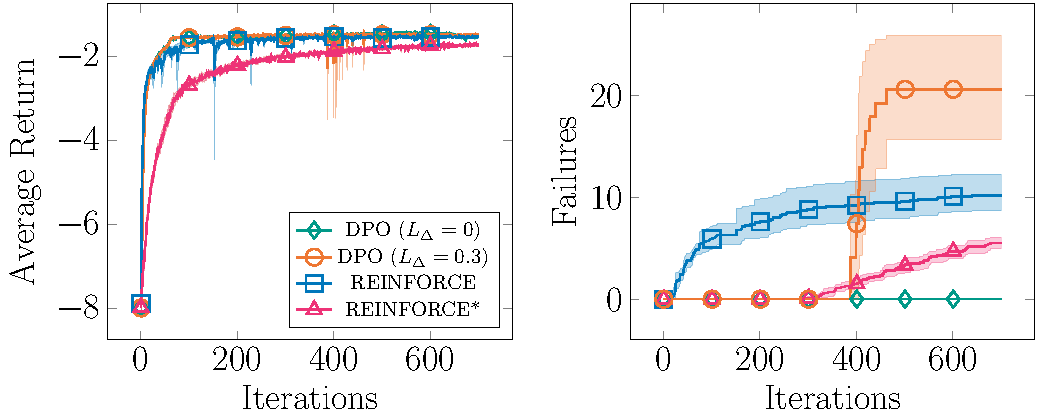
\includegraphics[width=\columnwidth]{plots/minigolf.pdf}
	\caption{Minigolf results, averaged over $10$ random seeds with $95\%$ bootstrapped confidence intervals. On the left: average return ($\gamma=0.99$) per iteration. On the right: number of failing episodes in a batch of $500$ (the same legend applies).}
	\label{fig:minigolf}
\end{figure}

\subsection*{Task Specifications} 
The environment has a two-dimensional state and a scalar action. 
Both the state dimensions and the actions are represented with real values in the interval $[-1, 1]$. The arriving state $s'$ is computed with the following equation:
\begin{align}
s' &= As + Ba + \epsilon, \qquad \epsilon\sim\Gauss(0,\nu^2),\nonumber
\end{align}
where:
\begin{align}
&\quad A =
\begin{bmatrix}
1 & \tau \\
0 & 1 
\end{bmatrix}, &\quad 
B =
\begin{bmatrix}
0 \\
\frac{\tau}{mass} 
\end{bmatrix},\nonumber
\end{align}
$\nu=0.1$, $mass=1$ and $\tau = 1$.
Since the term $\epsilon$ is a Gaussian noise, $P(s'|s,a)$ will be a Gaussian distribution.
The reward function is:
\begin{align}
R(s) &= - (s^TQs + ara),\nonumber\\
\end{align}
where:
\begin{align}
Q =
\begin{bmatrix}
1 & 0 \\
0 & 0
\end{bmatrix},
\end{align}
and $r = 0.1 $.
The policy used for this task is linear in the state, with initial parameters = $[-0.3, -0.3]$. For \ac{PGPE}, a factored Gaussian hyper-policy $\Gauss(\boldsymbol{\rho},\mathop{diag}(\boldsymbol{\sigma}^2)$ is defined over the two-dimensional parameter space, where $\boldsymbol{\sigma}=e^{\boldsymbol{\omega}}$, $\boldsymbol{\rho},\boldsymbol{\omega}\in\Reals^2$ are learned parameters, and $\boldsymbol{\rho}$ is always initialized to $[-0.3,-0.3]$. Both the components of $\boldsymbol{\sigma}$ are initialized to the same scalar $\sigma$, selected as a hyper-parameter. 
We set a discount factor of $\gamma=0.95$ and a maximum task horizon of $20$ time steps.
%
\section{Robot Adaptation} \label{sec:safe}
Finally, we consider a more realistic scenario. A mobile robot on a flat surface has to reach goal areas specified by the user. 
The task is adapted from Safety Gym~\citep{ray2019benchmarking} and based on MuJoCo~\citep{todorov2012mujoco}. The robot has a speed-based actuator for turning and a force-based one for going forward and backward, resulting in a two-dimensional action. Its state is composed of typical sensor observations (accelerometer, velocimeter, gyroscope, magnetometer) and a compass pointing to the current goal, for a total of $9$ state variables. The goal is a randomly placed circular area, and the robot is rewarded for approaching it through a dense reward signal. Whenever reached, the goal is placed at a new random position. We initialize the robot with a good deterministic linear policy, learned with \ac{PGPE}, whose performance (averaged over $1000$ test episodes) is reported as a black dashed line in Figure~\ref{fig:recover}. Imagine this policy has been learned in a controlled environment, then the robot has been deployed in a facility where random actions are not permitted.\\
\newline
Then, a fault occurs, in the form of a fixed offset ($20\degree$) on the angle measured by the goal compass. The lower performance of the original policy after the fault is reported as a red dotted line in Figure~\ref{fig:recover}. A corresponding difference in the agent's behavior can be appreciated from the animation feature provided by MuJoCo to observe the simulation. Using \ac{DPO}, the agent can adapt the policy parameters to the environmental change, as shown in Figure~\ref{fig:recover}. The environment is deterministic. We also make the simplifying assumption $L_{\Delta}=0$ and show the results for a hand-tuned regularization parameter $\lambda$. For each policy update, a batch of $10$ episodes of $200$ steps each is collected, and we show the average return over each batch. The performance of \ac{PGPE} is also reported as a reference. Both algorithms are able to fine-tune the policy back to its original performance. However, \ac{DPO} does that without action randomization.

\begin{figure}[t]
	\begin{minipage}[t]{.48\columnwidth}
		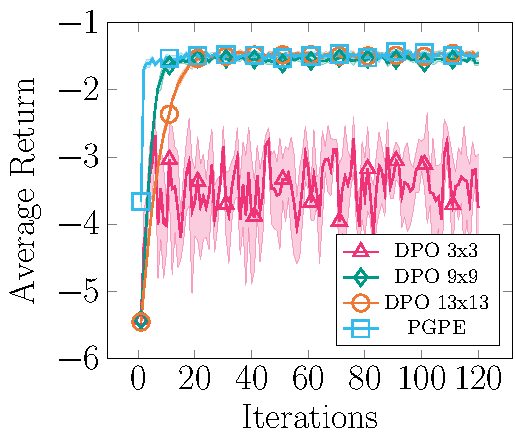
\includegraphics[width=\textwidth]{plots/mass.pdf}
		\caption{Double Integrator: average return ($\gamma=0.95$) per iteration, averaged over $5$ random seeds with $95\%$ bootstrapped confidence intervals.}
		\label{fig:mass}
	\end{minipage}%
	\hfill
	\begin{minipage}[t]{.48\columnwidth}
		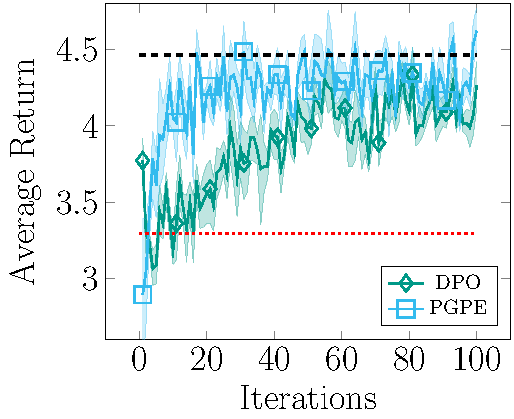
\includegraphics[width=\textwidth]{plots/recover.pdf}
		\caption{Robot Adaptation: average return (undiscounted) per iteration, averaged over $10$ random seeds with $95\%$ bootstrapped confidence intervals.}
		\label{fig:recover}
	\end{minipage}
\end{figure}

\subsection*{Task Specifications}
This is a custom environment built using the Safety Gym library~\citep{ray2019benchmarking}, which relies on the MuJoCo simulator~\citep{todorov2012mujoco}. The task is composed by a mobile robot that moves on a flat surface with the aim of reaching a randomly placed goal area. The state space considered in the task is composed by $9$ variables that represent the measurements of some sensors mounted on the robot. The robot is equipped with four standard sensors (accelerometer, velocimeter, gyroscope, magnetometer) and a compass that detects the orientation of the robot with regard to the goal area. Since the environment is flat, some of the data coming from the sensor (\eg vertical acceleration) are unnecessary and are simply discarded in order to reduce the dimensionality of the state space. 
The reduced state is composed by the following variables, reported here in the order in which they are considered in the implementation. All measurements are in the robot's frame of reference:
\begin{itemize}
	\item Linear acceleration in the plane (coordinates of a $2$D vector).
	\item Cosine and sine of the angle observed by the compass, which indicates the direction of the goal.
	\item Angular velocity of the robot (\wrt yaw);
	\item Magnetic flux observed by the magnetometer (coordinates of a $2$D vector).
	\item Linear velocity in the plane (coordinates of a $2$D vector).
\end{itemize}
Note that the robot has no information regarding its position in the world's frame of reference, which is not necessary for this task.
The reward function is defined as:
\[ 
R(s_t, a_t) = r \times \Delta distance\_from\_goal(t),
\]
where $r=1$, $\Delta distance\_from\_goal = distance(t) - distance(t-1)$ and $distance(t)$ measures the distance of the robot from the goal at time step $t$.
To compute $\Delta distance\_from\_goal$, the environment keeps a memory of previous distances. This, together with the fact that $distance(t)$ cannot be computed from the available observations, prevents us to compute $R(s,a)$ for all states and actions, as assumed in the paper. However, since $R(s_t,a_t)$ is independent from $a_t$, we can estimate $R(X,a)$ for any abstract state $X$ and action $a$ simply by averaging the rewards obtained in the states of $X$, regardless of the performed action. The delayed effect of actions on rewards is captured by also estimating the abstract transition function anyway.
For this task, we use a linear policy. The initial parameters, learned with \ac{PGPE} and representing an almost optimal policy before the compass fault, are reported here:
\[
\vtheta_{0} = 
\begin{bmatrix}
0.108& 0.022& 4.301& 0.108& 0.017& 0.112& 0.019& -0.179& -0.038\\
-0.004& 0.486& 0.105& -12.069& 1.070& -0.047& -0.222& 0.036& -0.398\\
\end{bmatrix}.
\]
For \ac{PGPE}, a factored Gaussian hyper-policy $\Gauss(\boldsymbol{\rho},\mathop{diag}(\boldsymbol{\sigma}^2))$ is defined over the $18$-dimensional parameter space, where $\boldsymbol{\sigma}=e^{\boldsymbol{\omega}}$, $\boldsymbol{\rho},\boldsymbol{\omega}\in\Reals^{18}$ are learned parameters, and $\boldsymbol{\rho}$ is initialized as $\vtheta_{0}$. All the components of $\boldsymbol{\sigma}$ are initialized to the same scalar $\sigma$, selected as a hyper-parameter.
We set a discount factor of $1$ and a maximum task horizon of $200$ ($2000$ in some experiments) time steps.


\section{Experimental Details}\label{sec:exp2}

In this section we provide further details on how the experiments presented in \mySec{sec:mini}, \mySec{sec:mass} and \mySec{sec:safe} were conducted. 

\subsection{Hyper-parameter tuning}
For each task, we have to tune some hyper-parameters before applying the different algorithms. We do so via \emph{grid search}. We define a set of reasonable values for these parameters and we fix a criterion for choosing the best parameters to be used in the algorithm. We compute the sum over $n$ iterations of the performance measure (estimated from the collected samples at each iteration of the algorithm) and average it over $m$ independent runs, performed with different random seeds. 
The values of $n$ and $m$ for the different experiments, together with other details, are reported in Table~\ref{tab:recap1}.
The results of the grid search are reported in Tables~\ref{tab:t1}-\ref{tab:t5}.
The bold values in the tables represent the combination of parameters used to perform the final experiments. For REINFORCE~\citep{williams1992simple}, the selected hyper-parameters are the step size $\alpha$ and the policy initial standard deviation $\sigma$. For \ac{DPO}, the learning rate $\alpha$ of the projection phase and the regularization coefficient $\lambda$ (see Section~\ref{sec:detail}). For \ac{PGPE}~\citep{sehnke2008policy}, the step size $\alpha$ and the hyper-policy initial standard deviation $\sigma$.

\begin{table}
	\centering
	\begin{tabular}{ll|cccccc}
		\toprule
		\textbf{Task} & \textbf{Algorithm} & $n$ & $m$ & $N$ & $H$ & $\gamma$ & $|\Xspace|$\\
		\midrule
		Minigolf & DPO & $300$ & $5$ & $500$ & 20 & $0.99$ & $12$ \\
		& REINFORCE & $300$ & $5$ & $500$ & 20 & $0.99$ & -- \\
		Double Integrator & DPO & $60$ & $3$ & $500$ & $20$ & $0.95$ & $9^{2}$ \\
		& PGPE & $100$ & $5$ & $500$ & $20$ & $0.95$ & -- \\
		Robot Adaptation & DPO & $500$ & $5$ & $1$ & $2000$ & $1$ & $5^{9}$ \\
		& PGPE & $100$ & $5$ & $10$ & $200$ & $1$ & --\\
		\midrule
	\end{tabular}
	\caption{\label{tab:recap1}Configurations used for hyper-parameter tuning. We denote with $n$ the number of iterations (policy updates), with $m$ the number of independent runs, with $N$ the batch size, with $H$ the task horizon, with $\gamma$ the discount factor and with $|\Xspace|$ the number of abstract states.}
\end{table}

\paragraph{Minigolf}
For REINFORCE (Table~\ref{tab:t2}) we performed the final experiment with two different combinations of parameters: $(\alpha=0.05, \log\sigma=-2)$ selected according to the criterion used in the tuning phase and $(\alpha=0.005, \log\sigma=-3)$, that provided the lowest number of \emph{failures} in the tuning phase.
\begin{table}[H]
	\centering
	\begin{tabular}{l|*{3}{c}}
		\toprule
		\backslashbox{$\alpha$}{$\lambda$}
		&0.0005&0.001&0.005\\
		\midrule
		0.001 & \textbf{-524.69} & -526.51 & -538.16 \\
		0.005 & -529.29 & -530.28 & -533.53 \\
		0.01 & -572.35 & -573.54 & -566.87 \\
		\bottomrule
	\end{tabular} \caption{\label{tab:t1} Grid search for \ac{DPO} on Minigolf.}
\end{table}
\begin{table}[H]
	\centering
	\begin{tabular}{l|*{3}{c}}
		\toprule
		\backslashbox{$\alpha$}{$\log\sigma$}
		&-4&-3&-2\\
		\midrule
		0.005 & -897.95 & \textbf{-883.72} & -876.55 \\
		0.01 & -1011.65 & -744.81 & -734.89 \\
		0.05 & -4971.86 & -2965.25 & \textbf{-551.86} \\
		\bottomrule
	\end{tabular} \caption{\label{tab:t2}Grid search for REINFORCE on Minigolf.}
\end{table}

\subsection*{Double Integrator} 
Hyper-parameter selection was performed for the $9\times 9$ discretization, and kept fixed in the final experiments for other discretizations. We used a fixed $\alpha$ (also for the next task) since its effects on performance are negligible. 
\begin{table}[H]
	\centering
	\begin{tabular}{l|*{3}{c}}
		\toprule
		\backslashbox{$\alpha$}{$\lambda$}
		&0.0001&0.0005&0.001\\
		\midrule
		0.025 & \textbf{-94.76} & -95.91 & -97.80 \\
		\bottomrule
	\end{tabular} \caption{\label{tab:t3}Grid search for \ac{DPO} on Double Integrator.}
\end{table}[H]
\begin{table}[H]
	\centering
	\begin{tabular}{l|*{3}{c}}
		\toprule
		\backslashbox{$\alpha$}{$\sigma$}
		&0.1&0.5&1\\
		\midrule
		0.1 & -187.86 & -184.57 & -190.18 \\
		0.5 & -174.69 & -158.39 & -161.64 \\
		1 & -169.29 & \textbf{-153.93}	 & -159.28 \\
		\bottomrule
	\end{tabular} \caption{\label{tab:t6}Grid search for \ac{PGPE} on Double Integrator.}
\end{table}

\subsection*{Robot Adaptation}
To verify the convergence of \ac{DPO}, we run it on a longer number of iterations than \ac{PGPE}. We also used a single, longer episode per iteration, which is more realistic. However, these settings were aligned for the final experiments, to make the comparison fair.
\begin{table}[H]
	\centering
	\begin{tabular}{l|*{3}{c}}
		\toprule
		\backslashbox{$\alpha$}{$\lambda$}
		&0.001&0.01&0.05\\
		\midrule
		0.005 & 20658.70 & 23163.38 & \textbf{23553.37} \\
		\bottomrule
	\end{tabular} \caption{\label{tab:t4}Grid search for \ac{DPO} on Robot Adaptation.}
\end{table}
\begin{table}[H]
	\centering
	\begin{tabular}{l|*{3}{c}}
		\toprule
		\backslashbox{$\alpha$}{$\sigma$}
		&0.1&0.5&1\\
		\midrule
		0.1 & 337.33 & 378.27 & 358.08 \\
		0.5 & 372.23 & 413.78 & 402.46 \\
		1 & 395.88 & \textbf{419.37}	 & 405.55 \\
		\bottomrule
	\end{tabular} \caption{\label{tab:t5}Grid search for \ac{PGPE} on Robot Adaptation.}
\end{table}

\subsection{Final Experiments}
The results of the final experiments (averaged over multiple runs performed with separate random seeds) are reported in the graphs in \mySec{sec:mini}, \mySec{sec:mass} and \mySec{sec:safe}. 
%Any differences among the algorithms on the same task (except from the selected hyper-parameters) that existed in the tuning phase were removed in the final experiments for fair comparison. 
We recap the final configurations in Table~\ref{tab:recap2} for the sake of reproducibility.

\begin{table}[H]
	\begin{tabular}{ll|ccccccccc}
		\toprule
		\textbf{Task} & \textbf{Alg} & $\alpha$ & $\lambda$ & $\sigma$ & $n$ & $m$ & $N$ & $H$ & \textbf{$\gamma$} & $|\Xspace|$\\
		\midrule
		Minigolf & DPO & $0.001$ & $0.0005$ & -- & $700$ & $10$ & $500$ & 20 & $0.99$ & $12$ \\
		& REIN. & $0.05$ & -- & $e^{-2}$ & $700$ & $10$ & $500$ & 20 & $0.99$ & -- \\
		& REIN.* & $0.005$ & -- & $e^{-3}$ & $700$ & $10$ & $500$ & 20 & $0.99$ & -- \\
		\midrule
		Double Int. & DPO & $0.025$ & $0.0001$ & -- & $120$ & $5$ & $500$ & $20$ & $0.95$ & $\{3^{2},9^{2},13^{2}\}$ \\
		& PGPE & $1$ & -- & $0.5$ & $120$ & $5$ & $500$ & $20$ & $0.95$ & -- \\
		\midrule
		Robot Ad. & DPO & $0.005$ & $0.05$ & -- & $100$ & $10$ & $10$ & $200$ & $1$ & $5^{9}$ \\
		& PGPE & $1$ & -- & $0.5$ & $100$ & $10$ & $10$ & $200$ & $1$ & --\\
		\midrule
	\end{tabular}
	\caption{\label{tab:recap2}Configurations used for hyper-parameter tuning, including hyper-parameters $\alpha$, $\lambda$ and $\sigma$. We denote with $n$ the number of iterations (policy updates), with $m$ the number of independent runs, with $N$ the batch size, with $H$ the task horizon, with $\gamma$ the discount factor and with $|\Xspace|$ the number of abstract states.}
\end{table}


\section{Additional Results}\label{sec:exp3}
In this section, we provide additional results on \ac{DPO}, with the purpose of better understanding its workings in practice. 

\subsection{Abstract state-space visualization in Robot Adaptation}
The Robot Adaptation task has a $9$-dimensional state space, discretized into a Cartesian grid of $5$ buckets per dimension. The total number of abstract states is very large ($\sim 10^{6}$) and could cause computational issues. However, as mentioned, only a subset of the abstract state space is actually visited by the agent and needs to be considered in the computations of \ac{DPO}. The colormaps of Figures~\ref{fig:cm0}-\ref{fig:cm99} show the visitation frequencies, for different iterations of the algorithm, of the abstract states, projected onto two of the most relevant state variables (the goal compass measurements) for visualization purposes. Axes labels are the bucket indexes, and the values are the ratios of total visits over $2000$ time steps, averaged over $10$ episodes. We can see that some abstract states are not visited at all. These are ignored in the estimation of the abstract transition and reward functions, in the value iteration phase and in the projection phase. Note how the visits change across iterations, and some previously ignored abstract states must be added to the abstract \ac{MDP}. The central states are never visited, as they correspond to unfeasible configurations (the two variables are the sine and cosine of an angle and their squares must always sum to one). We can also see an improvement in the agent's behavior: abstract state $(0,2)$ (the most visited one) corresponds to the agent facing the goal. After $99$ iterations, the visitation frequency of this state has significantly increased, meaning that the agent is able to point to the goal very quickly.

\subsection{Abstract policy visualization in Minigolf}
In Figures~\ref{fig:mg0}-\ref{fig:mg499} we visualize the policies (abstract and concrete) learned by \ac{DPO}, for different iterations of the Minigolf experiment. The plots have the original state space on the horizontal axis and the continuous action space on the vertical one (both are one-dimensional in this task). The red line represents the deterministic policy, which is linear in a vector of Gaussian radial-basis features (hence non-linear in the state). White boxes correspond to the $12$ abstract states and represent the restricted action space considered in the value iteration phase. Blue boxes represent the range of optimal actions obtained via value iteration. Note that, in this task, several optimal abstract policies exist. These are all considered as valid targets in the projection phase, in order to make the projection to the original policy space easier. The dotted line denotes the maximum action allowed by the environment (larger actions are clipped). When the box is placed above the dotted line, then, all the actions should be considered as optimal. This is not the case of the rightmost box in Figures~\ref{fig:mg399} and~\ref{fig:mg499}, where only a subset of the actions above the dotted line is considered as optimal. Indeed, by solving the task with $L_{\Delta}=0$, we assume that the friction has the same effect everywhere in the abstract state, which is not true in general. As a result, actions sampled where the friction is lower are evaluated better than they are.


\begin{figure}[h!]
	\centering
	\begin{minipage}[t]{.45\columnwidth}
		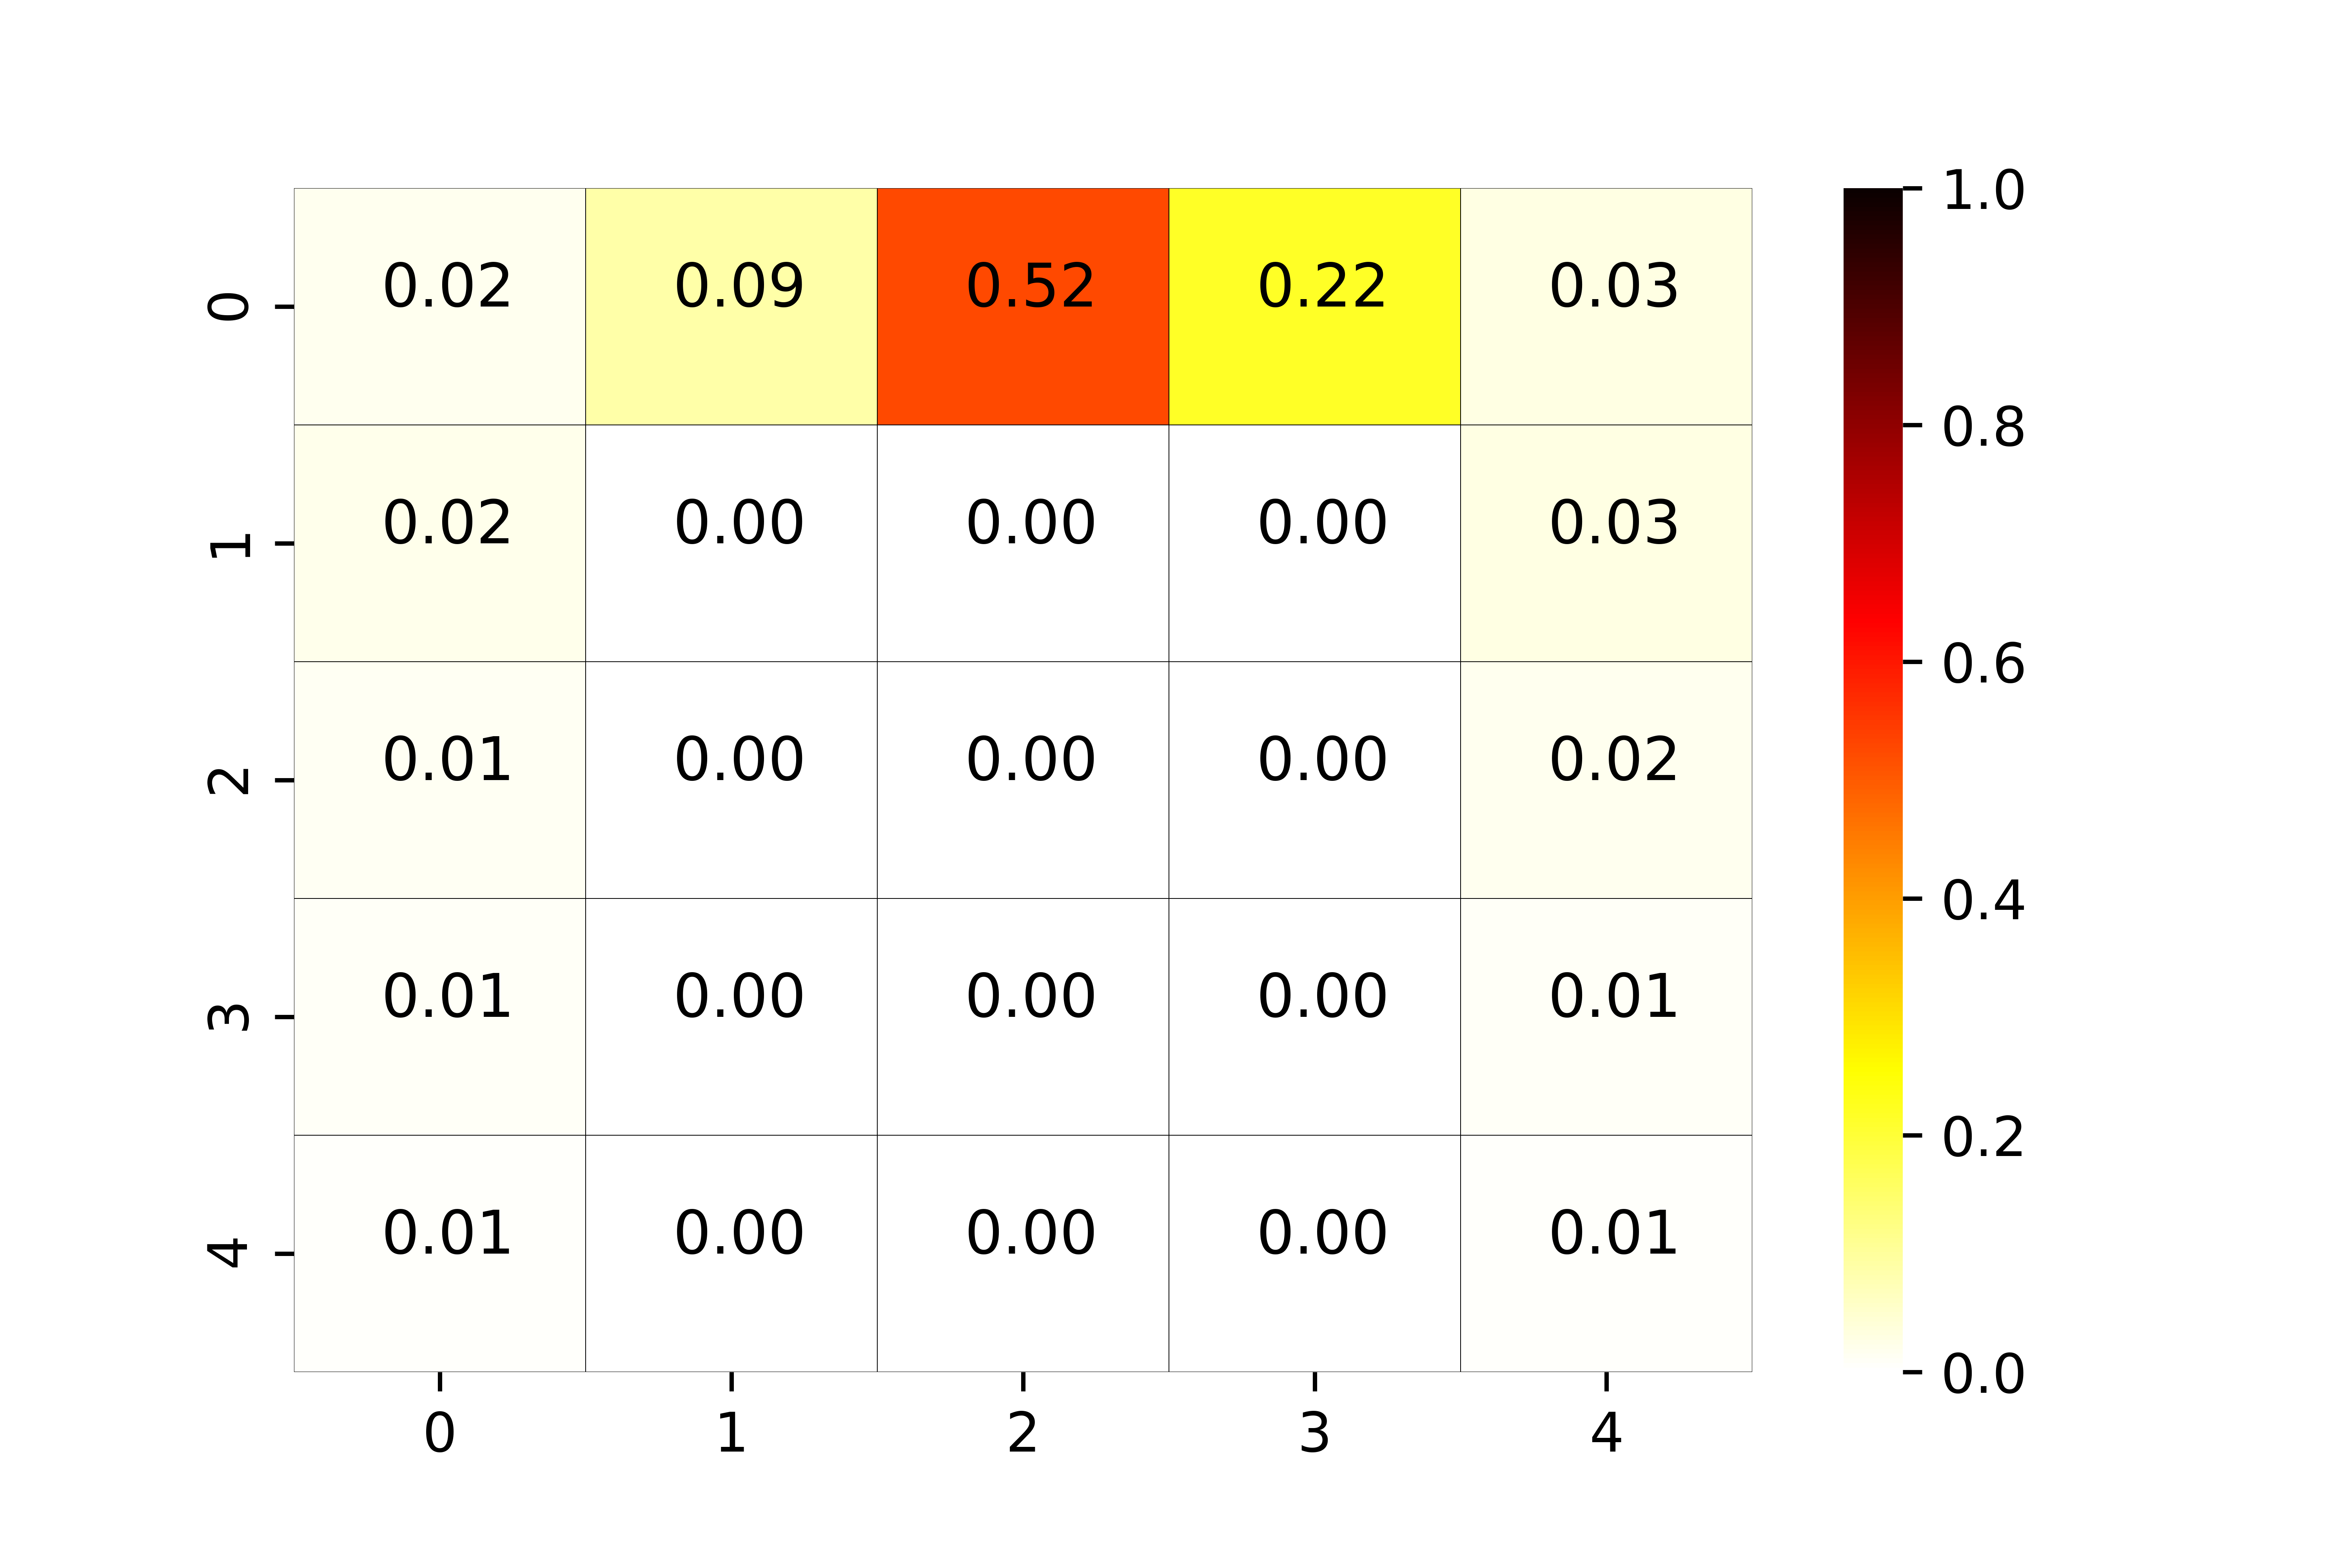
\includegraphics[width=\textwidth]{plots/colormap0.png}
		\caption{Robot Adaptation: abstract state visitation frequencies at the initial iteration of DPO.}
		\label{fig:cm0}
	\end{minipage}%
	\hfill
	\begin{minipage}[t]{.45\columnwidth}
		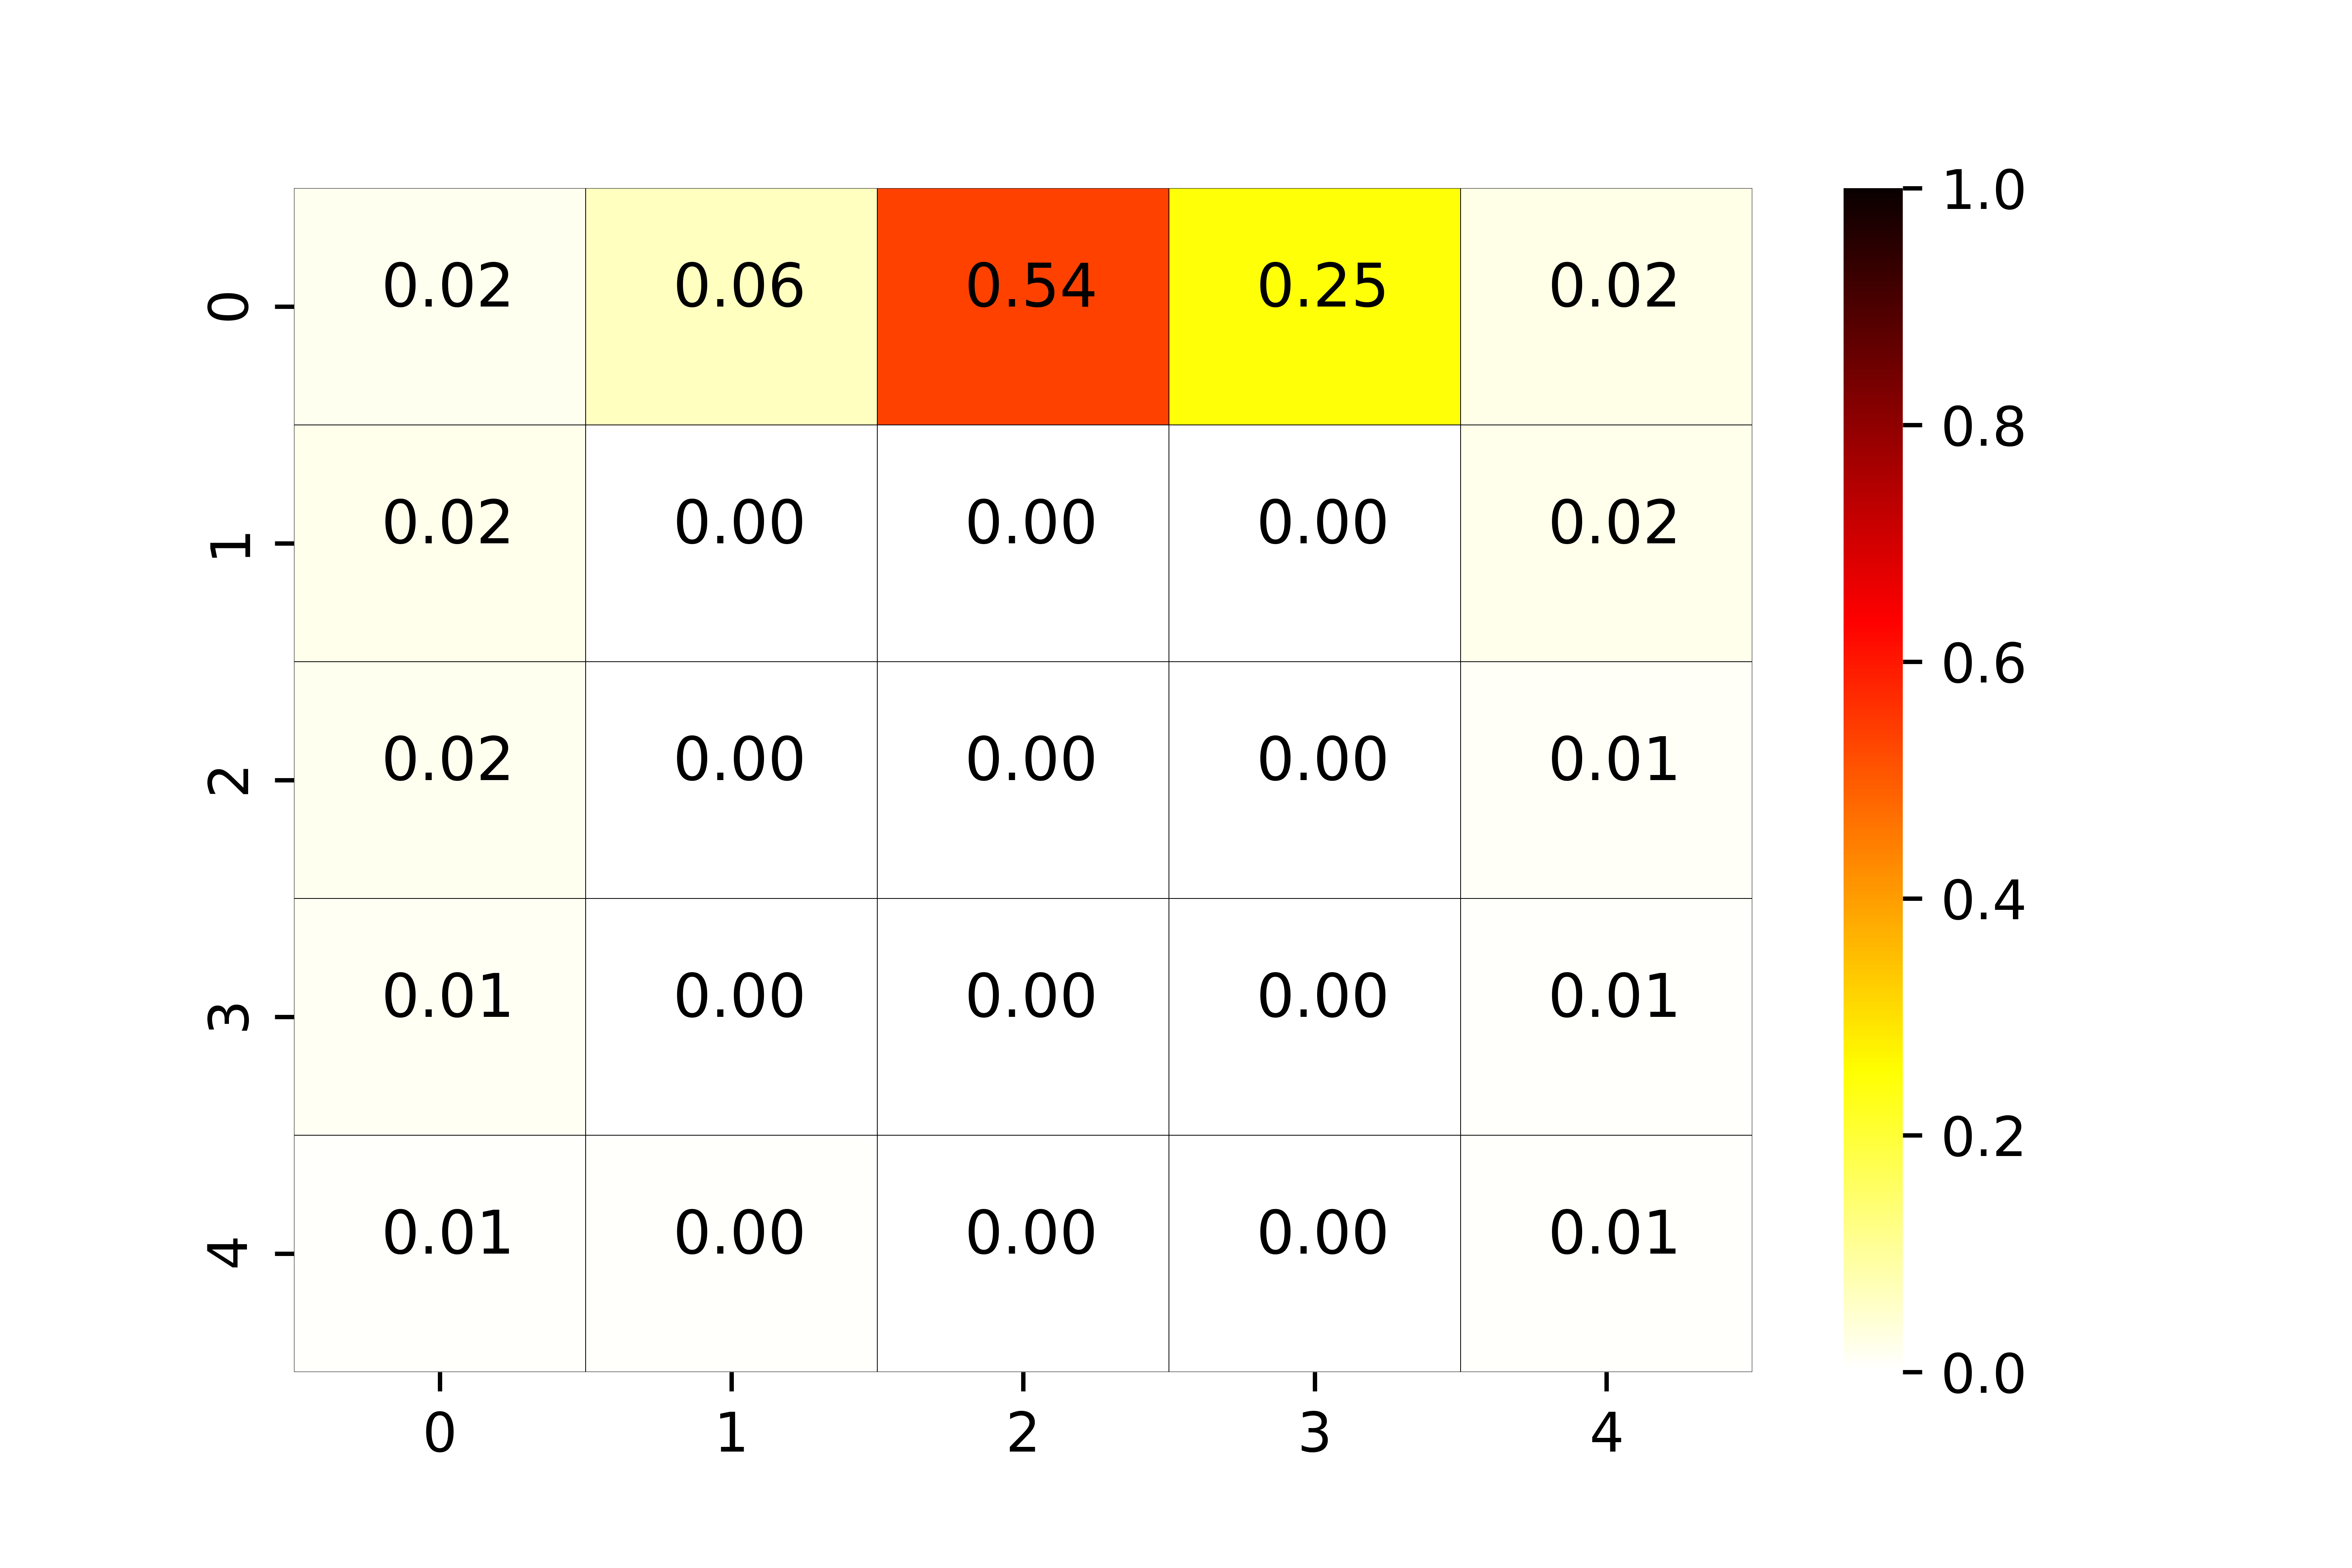
\includegraphics[width=\textwidth]{plots/colormap5.png}
		\caption{Robot Adaptation: abstract state visitation frequencies at the fifth iteration of DPO.}
		\label{fig:cm5}
	\end{minipage}
\end{figure}
\begin{figure}[h!]
	\centering
	\begin{minipage}[t]{.45\columnwidth}
		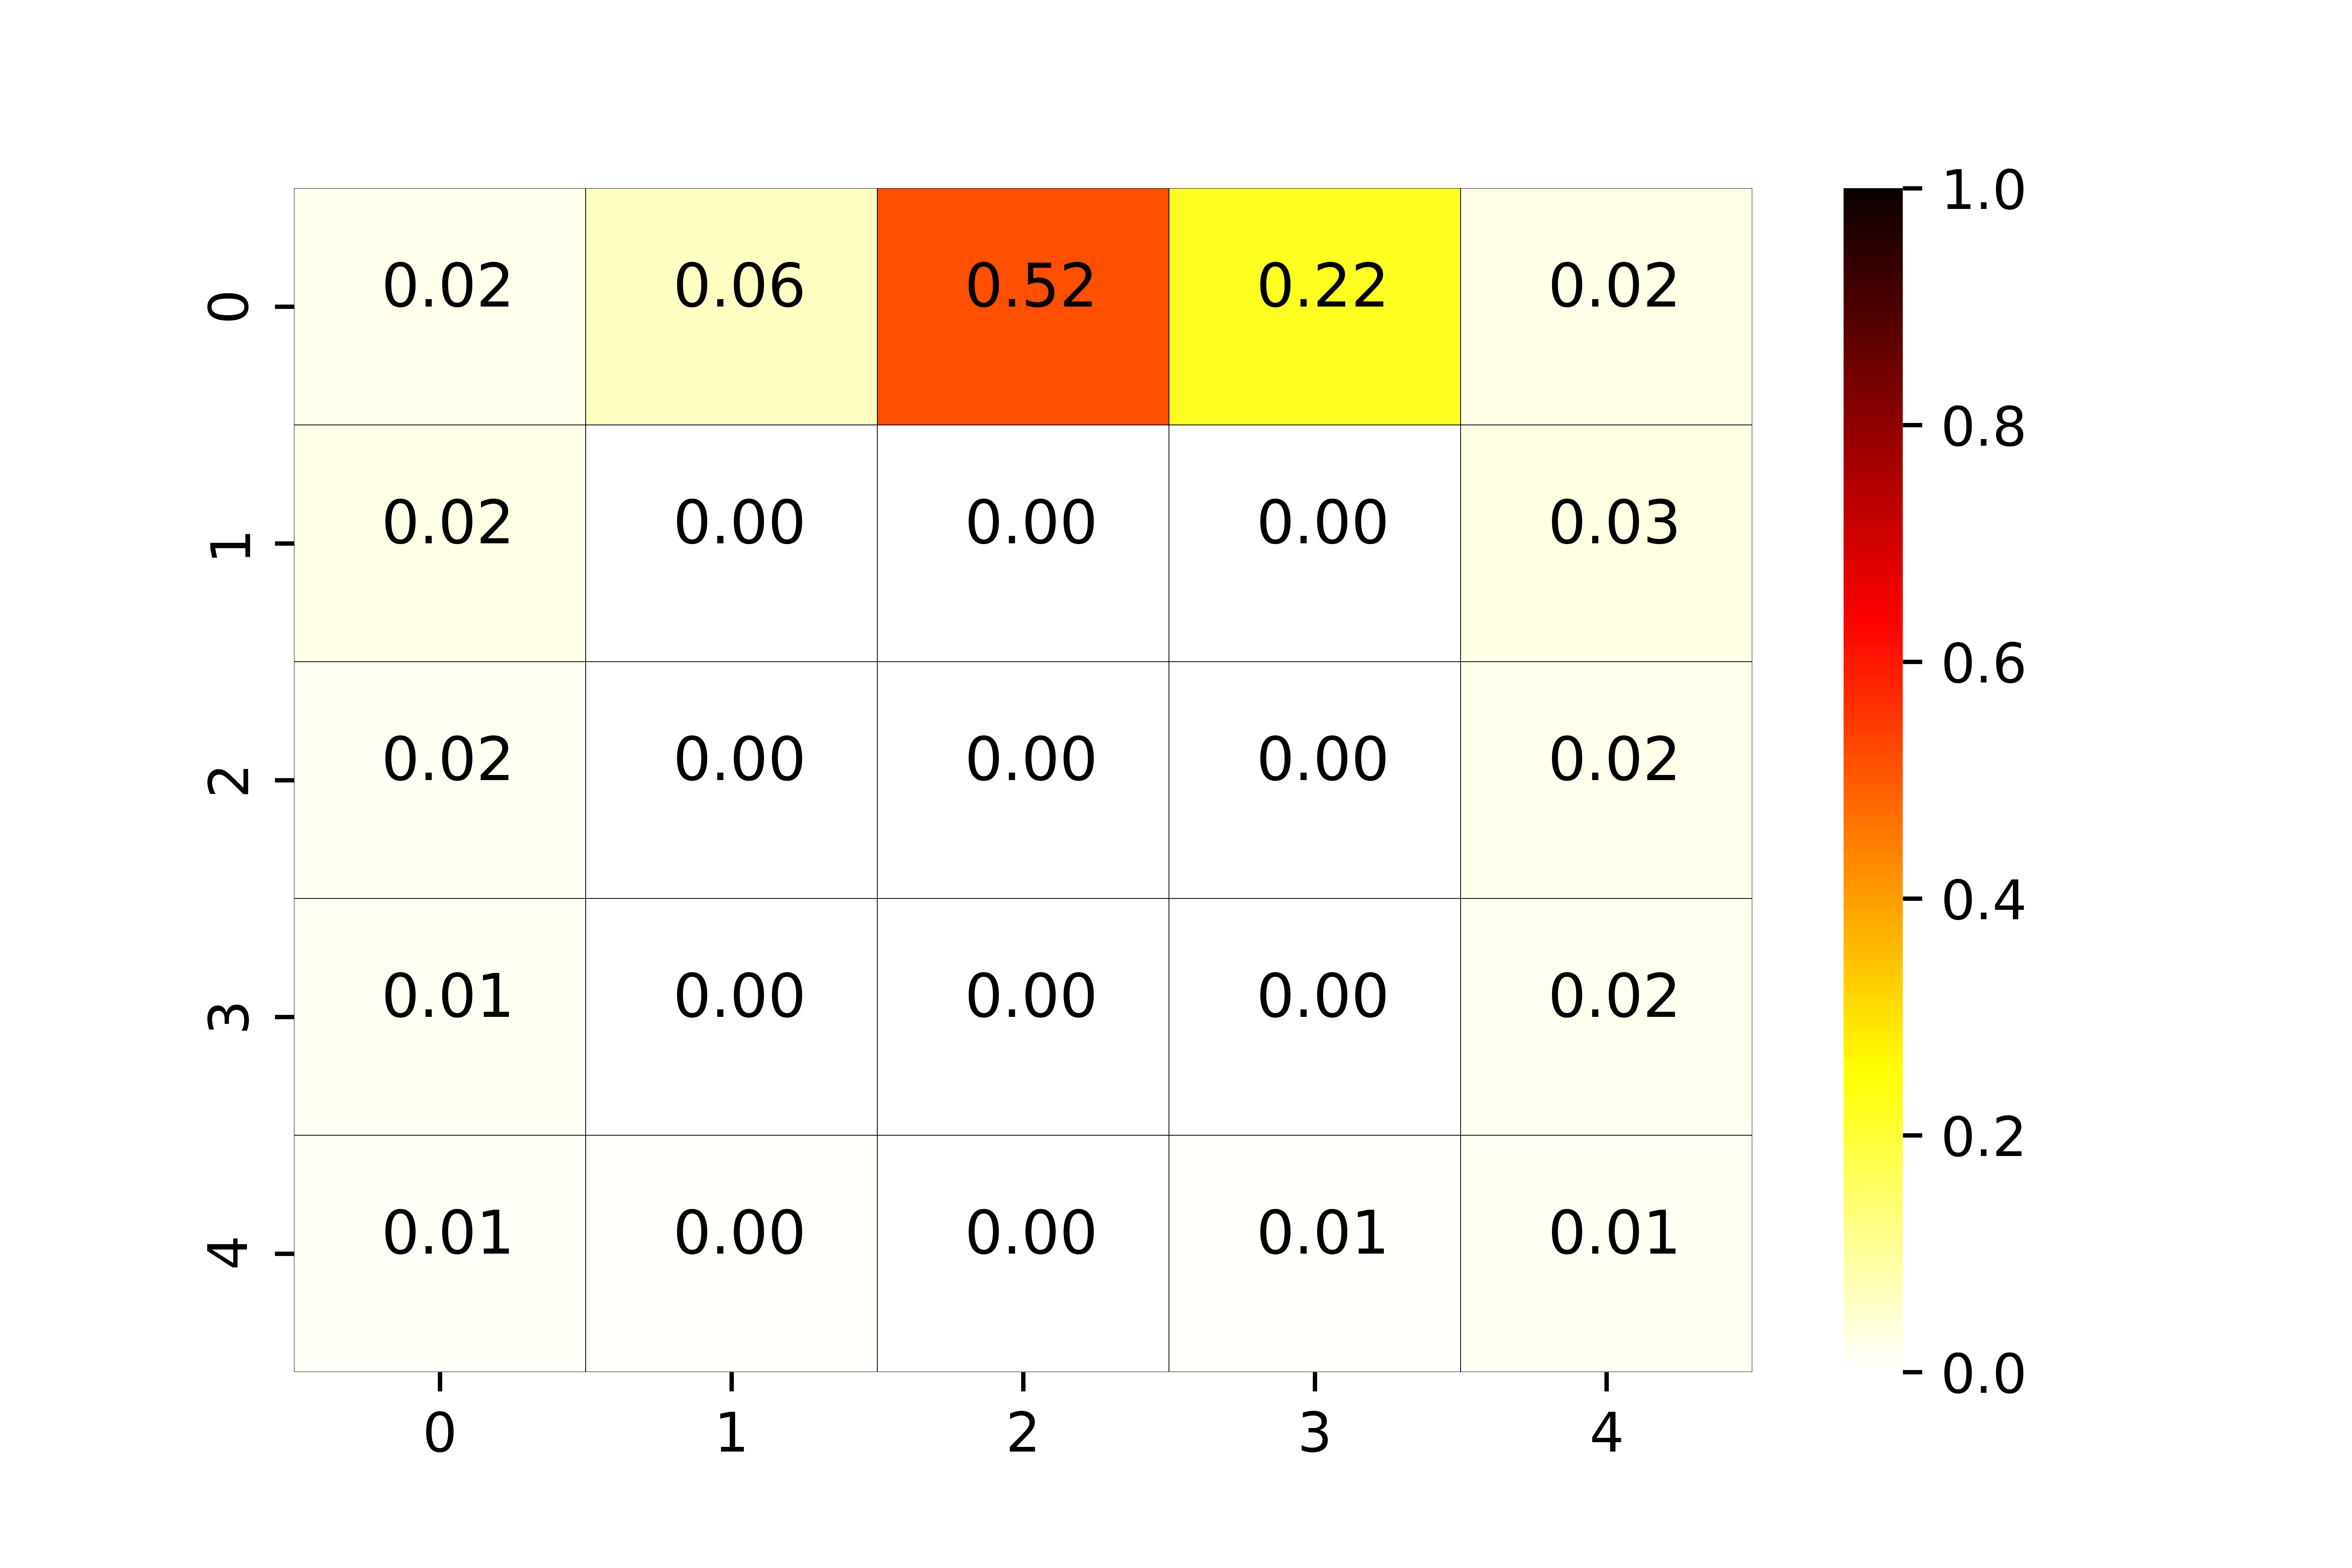
\includegraphics[width=\textwidth]{plots/colormap8.png}
		\caption{Robot Adaptation: abstract state visitation frequencies at the eighth iteration of DPO.}
		\label{fig:cm8}
	\end{minipage}%
	\hfill
	\begin{minipage}[t]{.45\columnwidth}
		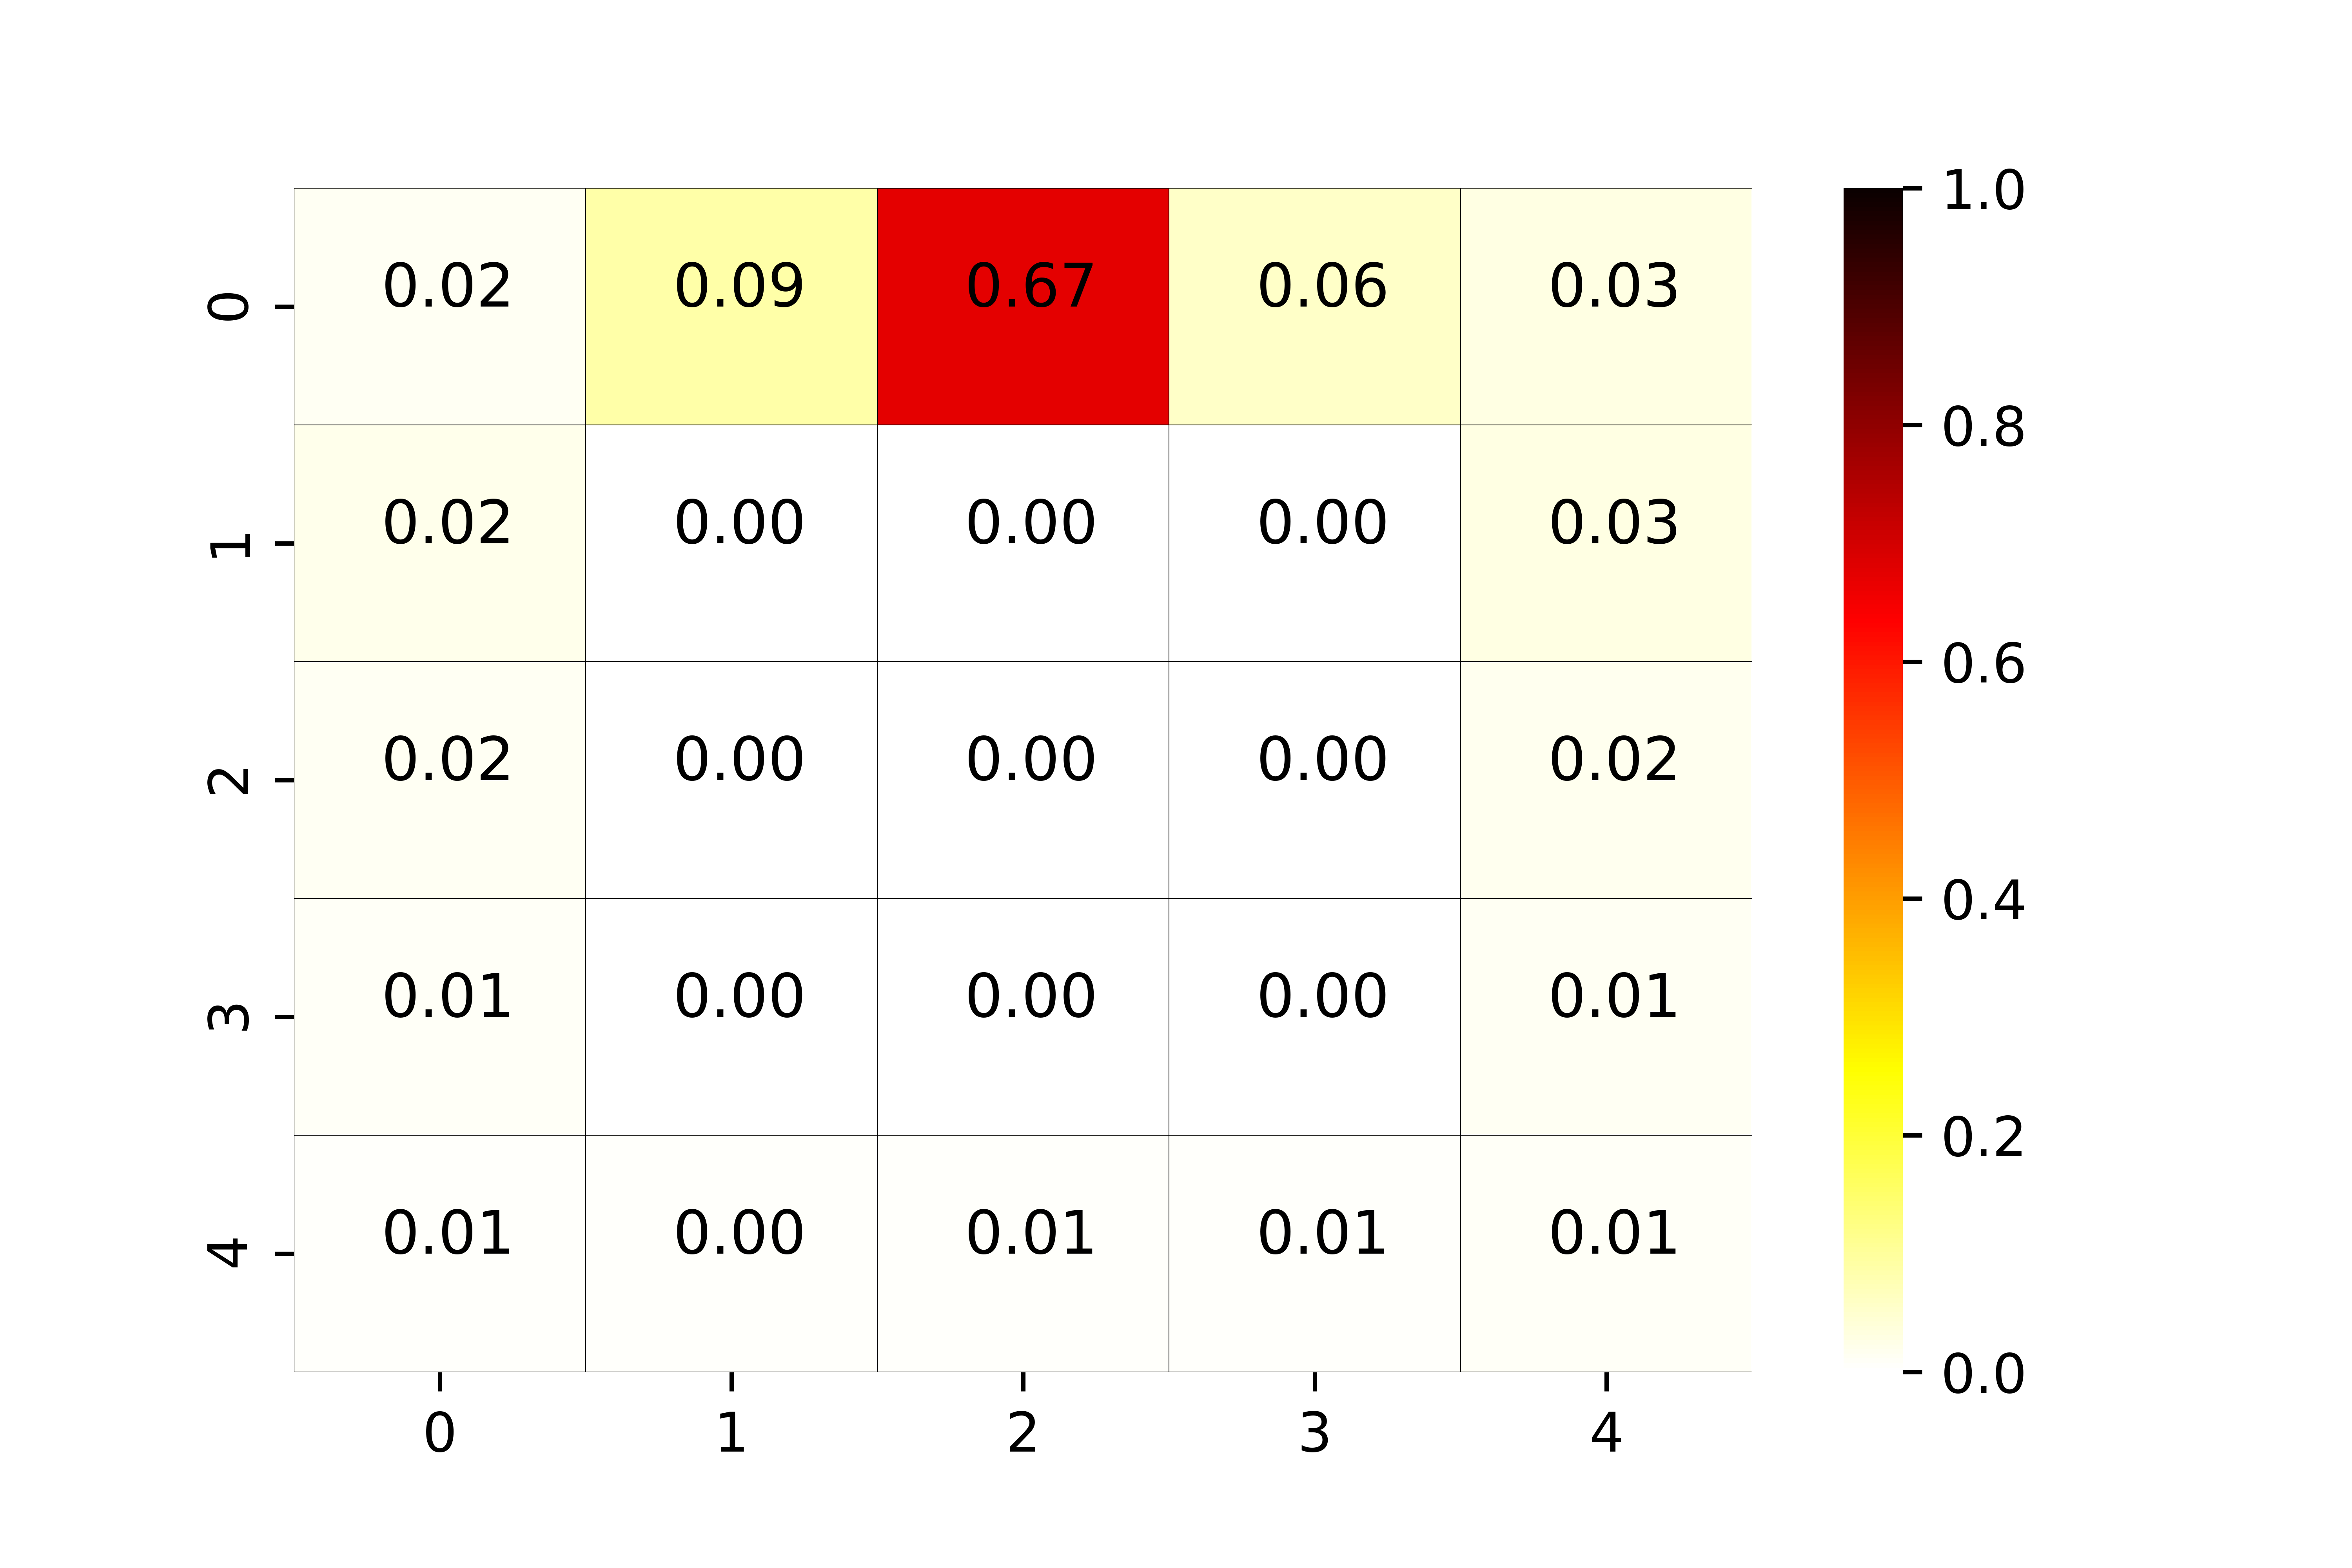
\includegraphics[width=\textwidth]{plots/colormap99.png}
		\caption{Robot Adaptation: abstract state visitation frequencies at the $99$-th (final) iteration of DPO.}
		\label{fig:cm99}
	\end{minipage}
\end{figure}

\begin{figure}[h!]
	\centering
	\begin{minipage}[t]{.48\columnwidth}
		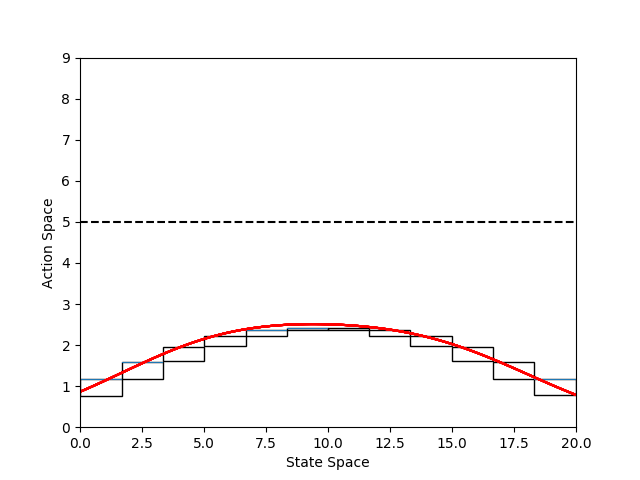
\includegraphics[width=\textwidth]{plots/it0.png}
		\caption{Minigolf: initial policy for DPO.}
		\label{fig:mg0}
	\end{minipage}%
	\hfill
	\begin{minipage}[t]{.48\columnwidth}
		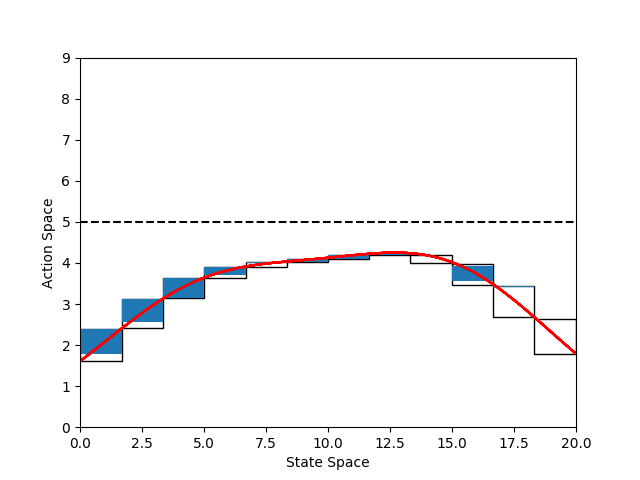
\includegraphics[width=\textwidth]{plots/it33.png}
		\caption{Minigolf: policy after $33$ iterations of DPO.}
		\label{fig:mg33}
	\end{minipage}
\end{figure}
\begin{figure}[h!]
	\centering
	\begin{minipage}[t]{.48\columnwidth}
		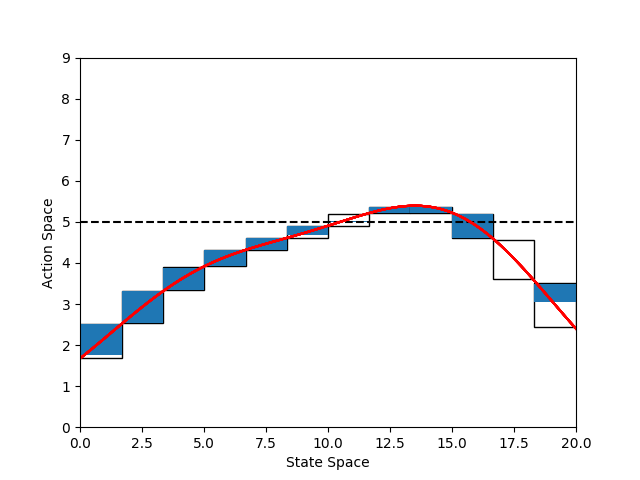
\includegraphics[width=\textwidth]{plots/it66.png}
		\caption{Minigolf: policy after $66$ iterations of DPO.}
		\label{fig:mg66}
	\end{minipage}%
	\hfill
	\begin{minipage}[t]{.48\columnwidth}
		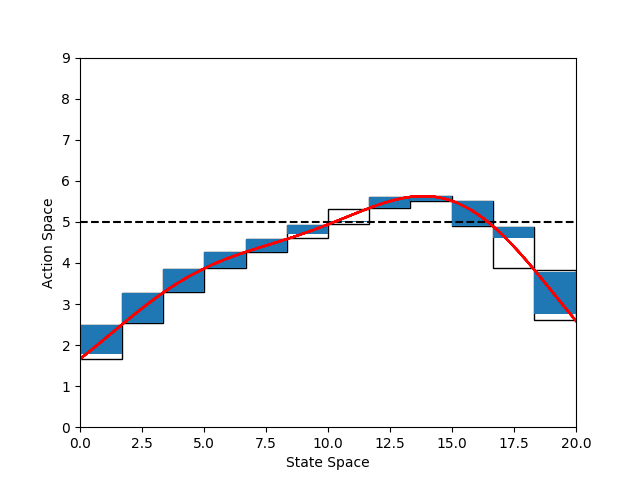
\includegraphics[width=\textwidth]{plots/it99.png}
		\caption{Minigolf: policy after $99$ iterations of DPO.}
		\label{fig:mg99}
	\end{minipage}
\end{figure}
\begin{figure}[h!]
	\centering
	\begin{minipage}[t]{.48\columnwidth}
		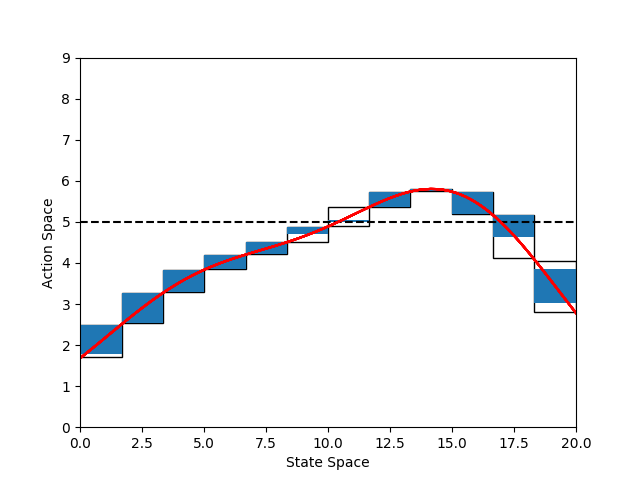
\includegraphics[width=\textwidth]{plots/it199.png}
		\caption{Minigolf: policy after $199$ iterations of DPO.}
		\label{fig:mg199}
	\end{minipage}%
	\hfill
	\begin{minipage}[t]{.48\columnwidth}
		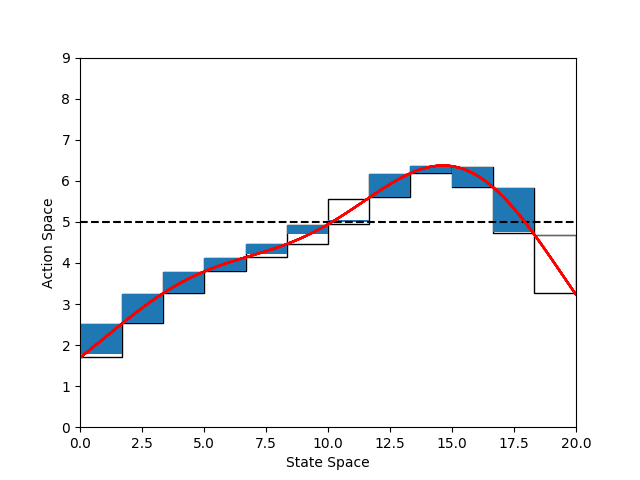
\includegraphics[width=\textwidth]{plots/it299.png}
		\caption{Minigolf: policy after $299$ iterations of DPO.}
		\label{fig:mg299}
	\end{minipage}
\end{figure}
\begin{figure}[h!]
	\centering
	\begin{minipage}[t]{.48\columnwidth}
		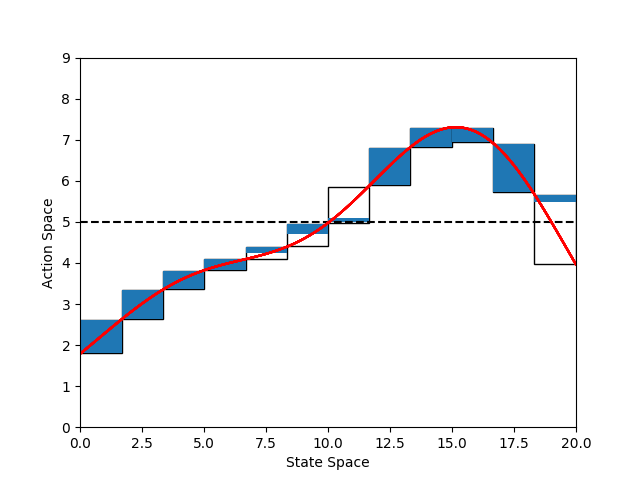
\includegraphics[width=\textwidth]{plots/it399.png}
		\caption{Minigolf: policy after $399$ iterations of DPO.}
		\label{fig:mg399}
	\end{minipage}%
	\hfill
	\begin{minipage}[t]{.48\columnwidth}
		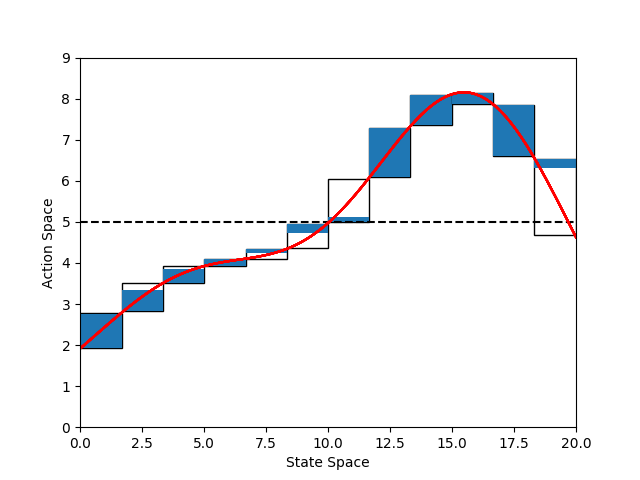
\includegraphics[width=\textwidth]{plots/it499.png}
		\caption{Minigolf: final policy after $499$ iterations of DPO.}
		\label{fig:mg499}
	\end{minipage}
\end{figure}

\clearpage